% r0, r1, r2, r3-1, r4-1, r4-1-2

\section{[R-0] Everyone <3 Fan Mail}

	This series of challenges were made slightly more tedious than necessary, because unfortunately there was a real company
	called \enquote{LightSpeed} that diluted the search results.

	The main objective of this challenge was to find the email of the site administrator for \url{www.lightspeedcorp.global}, and
	send him an email.

	\subsection{Solution}

		In theory, all we would have needed to do was perform a WHOIS lookup on the domain to find the email address. Simple,
		right?

		Nope.

		Depending on which WHOIS search engine is used, certain bits of information about the registrant can be missing if the
		domain was registered with WHOISGuard, which hides certain identifiable information from WHOIS lookups.

		\begin{figure}[!htbp]\centering
			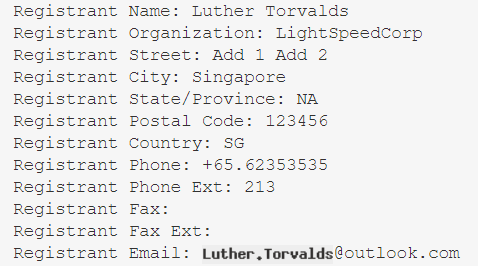
\includegraphics[width=110mm]{figures/osintred/r0.png} \vspace{5mm}
			\caption{All the information is visible if WHOISGuard is ignored}
		\end{figure}

		\pagebreak
		However, it turns out that the guard isn't perfect, and all we had to do was find a WHOIS search engine that ignores the
		guard. After some digging, we found one, exposing all the juicy details of the registrant.

		After getting the email address, we just had to send an email, and we were replied with the flag.

	% end subsection

	\subsection{Flag}
		The flag for this challenge was \cddcflag{IS\_IT\_I\_AM\_FAM0US\_NAO}.
	% end subsection

% end section


\pagebreak
\section{[R-1] Travel to the Past}

	The challenge heavily hinted that we would need a way to look at an older version of the website to find the flag, and that's exactly
	what we did.

	\subsection{Solution}

		There was a single snapshot of the website on the Wayback Machine\footnote{\url{https://archive.org/web/}} on the 20\sps{th} of May,
		and browsing that snapshot revealed the flag on the homepage of a blog:

		\begin{figure}[!htbp]\centering
			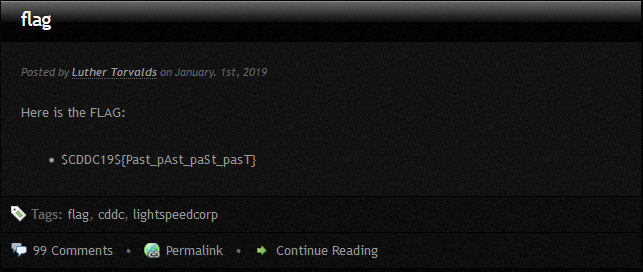
\includegraphics[width=110mm]{figures/osintred/r1.png} \vspace{5mm}
			\caption{The flag is clearly visible}
		\end{figure}

	% end subsection

	\subsection{Flag}
		The flag for this challenge was \cddcflag{Past\_pAst\_paSt\_pasT}.
	% end subsection

% end section


\pagebreak
\section{[R-2] I'm Sho Done With This}

	\subsection{Solution}

		The hint was in the question title itself --- turns out that there is a search engine called \enquote{ShoDan}
		\footnote{\url{https://www.shodan.io}}, which claims to be the world's first search engine for internet connected devices.

		Sure enough, searching for our favourite company \enquote{lightspeedcorp} yielded the following results:

		\begin{figure}[!htbp]\centering
			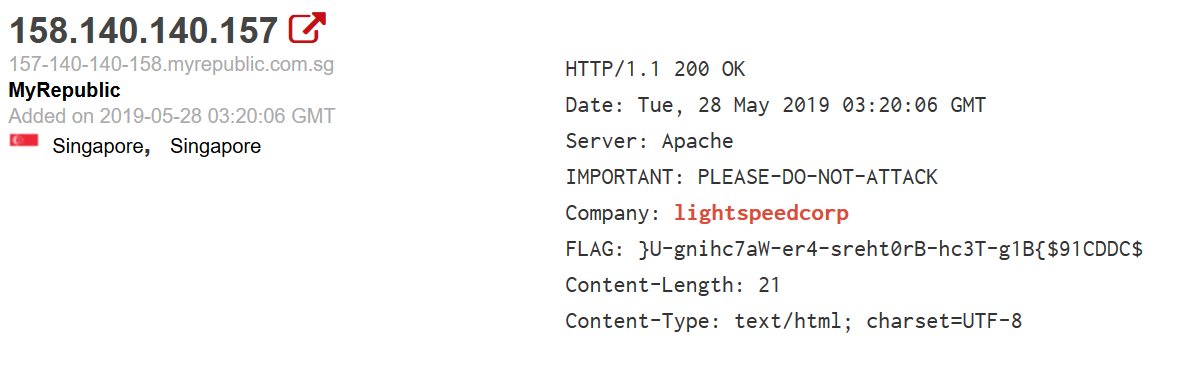
\includegraphics[width=150mm]{figures/osintred/r2.png} \vspace{5mm}
			\caption{The flag is reversed, for some reason}
		\end{figure}

		A trivial string-reverse later, the flag is obtained.

	% end subsection

	\subsection{Flag}
		The flag for this challenge was \cddcflag{B1g-T3ch-Br0thers-4re-Wa7ching-U}.
	% end subsection


% end section















